\documentclass[11pt]{amsart}
\usepackage{geometry}                % See geometry.pdf to learn the layout options. There are lots.
\geometry{a4paper}                   % ... or a4paper or a5paper or ...
%\geometry{landscape}                % Activate for for rotated page geometry
\usepackage[parfill]{parskip}    % Activate to begin paragraphs with an empty line rather than an indent
\usepackage{enumitem}
\usepackage{graphicx}
\usepackage{amssymb}
\usepackage{amsmath}
\usepackage{cancel}
\usepackage{epstopdf}
\DeclareGraphicsRule{.tif}{png}{.png}{`convert #1 `dirname #1`/`basename #1 .tif`.png}
\usepackage{breqn}
\usepackage{float}
\usepackage{breqn}

\title{Econ 210C Problem Set \# 5}
\author{Minki Kim}
%\date{}                                           % Activate to display a given date or no date

\begin{document}




\maketitle

\section{Problems from Romer}
\subsection{Romer, Problem 6.13.}
\begin{enumerate}[label = (\alph*)]
	\item Think of an asset that pays $-c$ per unit time when the individual climbs a tree and $\bar{u}$ when the worker is unemployed. 
	In addition, assume that the asset is being priced by risk-neutral investors with required rate of return $r$. 
	Since the expected present value of lifetime dividends of this asset is the same as the individual's expected present value of lifetime utility, the asset's price must be $V_P$ when the individual is looking for palm trees and $V_C$ when the individual is looking for people with coconuts. 
	For the asset to be held, it must provide an expected rate of return of $r$. 
	That is, its dividends per unit time, plus any expected capital gains or losses per unit time, must equal $rV_P$.
	When the individual is looking for trees, there are no dividends, whereas there is a payoff of $V_C - V_P - c$ when the individual finds a tree and climbs it (which occurs with probability $b$). 
	Thus,
	\[
	r V_P = b(V_C - V_p - c)
	\]

	\item If the individual is looking for others with coconuts, there are no dividends, whereas there is a payoff of $V_P - V_C + \bar{u}$ when someone with a coconut is found, which occurs with probability $aL$.
	Thus,
	\[
	rV_C = a L (V_P - V_C + \bar{u})
	\]
	\item Substituting the equation from part a into the equation from part b yields
	\[
	V_P = \frac{rV_C}{aL} + V_C - \bar{u} \implies r \times \left(\frac{rV_C}{aL} + V_C - \bar{u}\right) = b \times \left(\frac{rV_C}{aL} + \bar{u} - c\right)
	\]
	which gets us
	\[
	V_C \times \left(\frac{r^2 + r a L + r b}{a L}\right) = \bar{u} (r+b) - bc
	\]
	so we have
	\[
	V_C = \frac{a L ( \bar{u} (r+b) - bc)}{r^2 + r a L + r b}
	\]
	and substituting in gets us
	\[
	V_P = \frac{\bar{u} (r+b) - bc}{r + a L + b} + \frac{a L ( \bar{u} (r+b) - bc)}{r^2 + r a L + r b} - \bar{u}
	\]
	so we can subtract and simplify to get our final answer
	\[
	V_C - V_P = \frac{bc + a L \bar{u}}{r + a L + b}
	\]
	\item We have the condition
	\[
	a L \times L = b \times (N - L)
	\]
	which is a quadratic in $L$ that we can use the quadratic formula for (ignoring the negative solution)
	\[
	L = \frac{-b + \sqrt{b^2 + 4 a b N}}{2a}
	\]
	and use the given substitution to obtain
	\[
	L = \frac{-b + \sqrt{9b^2}}{2a} = \frac{b}{a}
	\]
	\item We need the cost of climbing to be worthwhile, implying the condition
	\[
	V_C - V_P \geq c
	\]
	but we already have a closed form for $V_C - V_P$ we can use and apply our substitution to, so we have
	\[
	\frac{b c + b \bar{u}}{r + 2 b} \geq c
	\]
	and so we can solve for the constraint on c to get
	\[
	c \leq \frac{b \bar{u}}{r + b}
	\]
	for the possible values of $c$.
	\item It is a best response for no one to climb when no one else climbs (since no trade will occur) as long as climbing is costly, that is when $c > 0$. 
	So any positive $c$ gives an equilibrium where $L = 0$. 
	From earlier, we have the other equilibrium of $L = \frac{b}{a}$ when 
	\[
	0 < c \leq \frac{b \bar{u}}{r + b}
	\]
	so this range does imply multiple equilibria.
	The equilibrium with positive $L$ has higher welfare, which must be the case for climbing to be worthwhile (every climb gives a positive payoff relative to the no climbing case so more climbing means more overall payoff).
	
\end{enumerate}
\subsection{Romer, Problem 7.10.}

We have average price in each time period
\[
p_t = (1-\alpha) (p_{y-1} + \gamma \pi_{t-1}) + \alpha x_t
\]
Subtract last period's price from both sides
\[
p_t - p_{t-1} = (1-\alpha) \gamma \pi_{t-1} + \alpha (x_t - p_{t-1})
\]
Expand the right side
\[
p_t - p_{t-1} = (1-\alpha) \gamma \pi_{t-1} + \alpha (x_t  - p_t + p_t - p_{t-1})
\]
Substitute
\[
\pi_t = (1-\alpha) \gamma \pi_{t-1} + \alpha (x_t  - p_t + \pi_t)
\]
Rearrange to get
\[
x_t - p_t = \frac{1-\alpha}{\alpha} \times (\pi_t - \gamma \pi_{t-1})
\]

We now have a new problem for the firm
\[
\min_{x_t} \frac{1}{2} \times (x_t - (p_t + \phi y_t))^2 + \sum_{j=1}^{\infty} \beta^j (1-\alpha)^j  \frac{1}{2} E_t \left( x_t + \sum_{k=0}^{j-1} \gamma \pi_{t+k} - \left[ p_t + \sum_{k=1}^j \pi_{t+k} + \phi y_{t+j} \right] \right)^2
\]
since firms have to set a price today that can cause them a loss today, but they also have to take into account the future, which is both discounted (accounted for with the $\beta$ term) and where they may be able to adjust prices anyway (hence the $1-\alpha$ term).
The partial indexation means that the price in period $t$ is the previous period's price plus $\gamma \pi_{t-1}$, so we account for all of these changes with the $x_t + \sum_{k=0}^{j-1} \gamma \pi_{t+k}$ term.
The profit maximizing price in the future is accounted for with the $p_t + \sum_{k=1}^j \pi_{t+k} + \phi y_{t+j}$ term.

Now we solve the firm's problem using the first order condition
\[
x_t - (p_t + \phi y_t) + \sum_{j=1}^{\infty} \beta^j (1-\alpha)^j E_t \left( x_t + \sum_{k=0}^{j-1} \gamma \pi_{t+k} - \left[ p_t + \sum_{k=1}^j \pi_{t+k} + \phi y_{t+j} \right] \right) = 0
\]
Now we want to get a geometric series to simplify, but we can't do that with terms inside the expectation. 
However, the $x_t$ and $p_t$ terms inside the expectation are chosen and known today, so we can pull them out of the expectation and have a new summation to simplify as follows
\[
\left[ \sum_{j=0}^{\infty} [\beta \times (1-\alpha)]^j x_t - p_t \right] -\phi y_t +  \sum_{j=1}^{\infty} \beta^j (1-\alpha)^j E_t \left( \sum_{k=0}^{j-1} \gamma \pi_{t+k} - \left[ \sum_{k=1}^j \pi_{t+k} + \phi y_{t+j} \right] \right) = 0
\]
so we can use the formula for an infinite geometric series to get
\[
\frac{x_t - p_t}{1 - \beta (1-\alpha)} - \phi y_t +  \sum_{j=1}^{\infty} \beta^j (1-\alpha)^j E_t \left( \sum_{k=0}^{j-1} \gamma \pi_{t+k} - \left[ \sum_{k=1}^j \pi_{t+k} + \phi y_{t+j} \right] \right) = 0
\]
which we can iterate forward one period to get
\[
E_t \frac{x_{t+1} - p_{t+1}}{1 - \beta (1-\alpha)} - \phi E_t y_{t+1} +  \sum_{j=2}^{\infty} \beta^j (1-\alpha)^j E_t \left( \sum_{k=1}^{j-1} \gamma \pi_{t+k} - \left[ \sum_{k=2}^j \pi_{t+k} + \phi y_{t+j} \right] \right) = 0
\]
and we now have a new substitution of the form
\[
E_t [x_{t+1} - p_{t+1}] = \phi E_t y_{t+1} - \sum_{j=2}^{\infty} \beta^j (1-\alpha)^j E_t \left( \sum_{k=1}^{j-1} \gamma \pi_{t+k} - \left[ \sum_{k=2}^j \pi_{t+k} + \phi y_{t+j} \right] \right)
\]
which accounts for all but a few of the terms in the 
\[
\sum_{j=1}^{\infty} \beta^j (1-\alpha)^j E_t \left( \sum_{k=0}^{j-1} \gamma \pi_{t+k} - \left[ \sum_{k=1}^j \pi_{t+k} + \phi y_{t+j} \right] \right)
\]
expression.
The $j=1$ term
\[
\beta (1-\alpha) E_t \left( \gamma \pi_{t} - \left[ \pi_{t+1} \right] \right)
\]
along with the $k=0$ parts of the $j>1$ terms for partial indexation
\[
\sum_{j=2}^{\infty}\beta^j (1-\alpha)^j \gamma \pi_t 
\]
and the $k=1$ parts of the $j>1$ terms for the future profit maximizing prices
\[
- \sum_{j=2}^{\infty} \beta^j (1-\alpha)^j \pi_{t+1}
\]
remain.

So after moving $x_t - p_t$ to the left, we are left with
\begin{align*}
x_t - p_t = &(1 - \beta (1-\alpha)) \left[\phi y_t - \beta (1-\alpha) (\gamma \pi_{t} - \pi_{t+1}) + \sum_{j=2}^{\infty} \beta^j (1-\alpha)^j E_t \left\{ - \gamma \pi_t  + \pi_{t+1} \right\} \right] \\ &+ \beta (1-\alpha) E_t [x_{t+1} - p_{t+1}]
\end{align*}
and we can rewrite this as
\[
x_t - p_t = (1 - \beta (1-\alpha)) \left[\phi y_t + \sum_{j=1}^{\infty} \beta^j (1-\alpha)^j E_t \left\{ - \gamma \pi_t  + \pi_{t+1} \right\} \right] + \beta (1-\alpha) E_t [x_{t+1} - p_{t+1}]
\]
which we can apply the geometric series formula to and obtain
\[
x_t - p_t = (1 - \beta (1-\alpha)) \left[\phi y_t + \frac{\beta \times (1-\alpha)}{1 - \beta \times (1-\alpha)} E_t \left\{ - \gamma \pi_t  + \pi_{t+1} \right\} \right] + \beta (1-\alpha) E_t [x_{t+1} - p_{t+1}]
\]
which we can simplify to 
\[
x_t - p_t = (1 - \beta (1-\alpha)) \phi y_t + \beta (1-\alpha) \left\{ - \gamma \pi_t + E_t \pi_{t+1} + E_t [x_{t+1} - p_{t+1}] \right\}
\]
which is another formula for $x_t - p_t$ now available. So we have
\[
 \frac{1-\alpha}{\alpha} \times (\pi_t - \gamma \pi_{t-1}) = (1 - \beta (1-\alpha)) \phi y_t + \beta (1-\alpha) \left\{ - \gamma \pi_t + E_t \pi_{t+1} + E_t [x_{t+1} - p_{t+1}] \right\}
\]
and we can iterate the earlier formula forward to get the substitution
\[
E_t[x_{t+1} - p_{t+1}] = \frac{1-\alpha}{\alpha} \times E_t(\pi_{t+1} - \gamma \pi_{t})
\]
giving us
\[
 \frac{1-\alpha}{\alpha} \times (\pi_t - \gamma \pi_{t-1}) = (1 - \beta (1-\alpha)) \phi y_t + \beta (1-\alpha) \left\{ - \gamma \pi_t + E_t \pi_{t+1} + \frac{1-\alpha}{\alpha} \times E_t(\pi_{t+1} - \gamma \pi_{t}) \right\}
\]
which simplifies as
\[
\frac{1-\alpha}{\alpha} \times (\pi_t - \gamma \pi_{t-1}) = (1 - \beta (1-\alpha)) \phi y_t + \beta \times \frac{1-\alpha}{\alpha} \left\{ - \gamma \pi_t + E_t \pi_{t+1} \right\}
\]
which we now want to solve for $\pi_t$ to get the Phillips curve.
So we can collect terms on either side to get
\[
\frac{1-\alpha}{\alpha} \times \pi_t + \beta \times \frac{1-\alpha}{\alpha} \gamma \pi_t = (1 - \beta (1-\alpha)) \phi y_t + \beta \times \frac{1-\alpha}{\alpha} E_t \pi_{t+1} + \frac{1-\alpha}{\alpha} \gamma \pi_{t-1}
\]
and collect coefficients on the left to have
\[
\pi_t \times \frac{1-\alpha}{\alpha} \times (1 + \beta \gamma) = (1 - \beta (1-\alpha)) \phi y_t + \beta \times \frac{1-\alpha}{\alpha} E_t \pi_{t+1} + \frac{1-\alpha}{\alpha} \gamma \pi_{t-1}
\]
and finally we simplify to get
\[
\pi_t = \frac{1}{1 + \beta \gamma}  \times \frac{\alpha}{1-\alpha} \times (1 - \beta (1-\alpha)) \phi y_t + \frac{\beta}{1 + \beta \gamma}E_t \pi_{t+1} +  \frac{1}{1 + \beta \gamma} \gamma \pi_{t-1}
\]
as our answer.

When $\gamma = 0$, we have just
\[
\pi_t =  \frac{\alpha}{1-\alpha} \times (1 - \beta (1-\alpha)) \phi  y_t +  \beta E_t \pi_{t+1} 
\]
which is indeed the new Keynesian Phillips curve.

When $\gamma = 0$, we have 
\[
\pi_t = \frac{1}{1 + \beta}  \times \frac{\alpha}{1-\alpha} \times (1 - \beta (1-\alpha)) \phi y_t + \frac{\beta}{1 + \beta}E_t \pi_{t+1} +  \frac{1}{1 + \beta} \pi_{t-1}
\]
which is indeed the new Keynesian Phillips curve with indexation.

\section{Quadratic cost of adjusting prices and effect of money \\ (Rotemberg 1982)}
\begin{enumerate}[label = (\alph*)]
	\item Convex costs of price adjustment fails to generate nominal stickiness of price changes. 
	Empirical evidence tells us that average duration of price change is about an year. 
	Continuously-changed price in this model is at odds with this fact. 
	However, convex cost can be calibrated to match the magnitude of the price changes, because large price changes are followed by increasing costs.

	\item 
	The choice of price today shows up both today and tomorrow. 
	So we have from the terms today and tomorrow the first order condition for $p_{i,t}$
	\[
	\cancel{2 \beta^t} (p_{i,t} - p_{i,t}^*) + \cancel{2 \beta^t} c (p_{i,t} - p_{i,t-1}) - \cancel{2 \beta^t} \beta c (E_t p_{i,t+1} - p_{i,t}) = 0
	\]
	The first order condition is: 
	\begin{equation*}
    p_{i,t} = \frac{1}{1 + c + \beta c} \left[ p_{i,t}^{*} + c p_{i,t-1} + c \beta E_t p_{i,t+1} \right]
	\end{equation*}
<<<<<<< Updated upstream
	Assume the solution takes the form $p_{i,t} = \nu_{-1} p_{i,t-1} + \sum_{l=0}^{\infty}\nu_l \mathbb{E}_t [p_{i,t+l}^{*}]$.
	Then
=======
	which we can order 
	Assume the solution takes the form $p_{i,t} = \nu_{-1} p_{i,t-1} + \sum_{l=0}^{\infty}\nu_l \mathbb{E}_t [p_{i,t+l}^{*}]$. Then
>>>>>>> Stashed changes
	\begin{align*}
	p_{i,t+1} &= \nu_{-1} p_{i,t} + \sum_{l=0}^{\infty} \nu_l \mathbb{E}_t p_{i,t+l+1}^{*} \\
	& = \nu_{-1} \left( \nu_{-1} p_{i,t-1} + \sum_{l=0}^{\infty}\nu_l \mathbb{E}_t [p_{i,t+l}^{*}] \right)+ \sum_{l=0}^{\infty} \nu_l \mathbb{E}_t p_{i,t+l+1}^{*}
	\end{align*}
	
	Plugging this into the first order conditions and rearranging yields:
	\begin{dmath*}
		[1+c+\beta c] \nu_{-1} p_{i,t-1} + \sum_{l=0}^\infty \nu_l \left\lbrace 1+c+\beta c - \beta c \nu_{-1} \right\rbrace \mathbb{E}_t [p_{i,t+l}^*] = p_{i,t}^* + (c+\beta c \nu_{-1}^2) p_{i,t-1} + \beta c \sum_{l=0}^\infty  \nu_l \mathbb{E}_t [p_{i,t+1+l}^*]
	\end{dmath*}
	Match the coefficients on $p_{i,t-1}$, $p_{i,t}^*$, and $p_{t+l}^*$ to get
	\begin{align*}
		&(1 + c + \beta c) \nu_{-1} = c + \beta c \nu_{-1}^2 \\
		&\nu_0 (1 + c + \beta c - \beta c \nu_{-1}) = 1 \\
		&\nu_{l+1} (1 + c + \beta c - \beta c \nu_{-1}) = \beta c \nu_l \hspace{0.1in} \text{for $l \geq 0$}
	\end{align*}
	Solving for $\nu_{-1}$ in the first equation using the quadratic formula yields
	\begin{equation*}
		\nu_{-1} = \frac{1}{2 \beta c} \left(1 + c + \beta c - \sqrt{(1 + c + \beta c)^2 - 4 \beta c ^2} \right)
	\end{equation*}
	where I choose the root that is smaller than 1. Using the remaining 2 equations, we get the rest of the coefficients:
	\begin{align*}
		&\nu_0 = \frac{1}{1 + c + \beta c - \beta c \nu_{-1}} \\
		&\nu_{l+1} = \frac{\beta c}{1 + c + \beta c - \beta c \nu_{-1}}
	\end{align*}

	\item
	Plugging the assumption into the first order condition yields and imposing symmetry, i.e., $p_{i,t} = p_t$, then rearranging yields
	\begin{equation*}
		[c + \beta c + \phi)] p_t = \phi m_t + c p_{t-1} + \beta c \mathbb{E}_t [p_{t+1}] 
	\end{equation*}
	Guess the solution takes the form
	\begin{equation*}
		p_t = \gamma_{-1} p_{t-1} + \sum_{l=0}^\infty \gamma_l \mathbb{E}_t m_{t+l}
	\end{equation*}
	Plug the guess into the first order condition and rearrange to obtain
	\begin{dmath*}
		(c + \beta c + \phi - \beta c \gamma_{-1}) \left[ \gamma_{-1} p_{t-1} + \sum_{l=0}^\infty \gamma_l \mathbb{E}_t [m_{t+l}] \right] = \phi m_t + c p_{t-1} + \beta c \sum_{l=0}^\infty \gamma_l \mathbb{E}_t [m_{t+1+l}]
	\end{dmath*}
	Match the coefficients on $p_{t-1}$, $m_t$, $m_{t+l}$ to get
	\begin{align*}
		&c = [c + \beta c + \phi - \beta c \gamma_{-1}] \\
		&\phi = \gamma_0 [c + \beta c + \phi - \beta c \gamma_{-1}] \\
		&\beta c \gamma_l = \gamma_{l+1} [c + \beta c + \phi - \beta c \gamma_{-1}] \hspace{0.1in} \text{for $l \geq 0$}
	\end{align*}
	Solving the quadratic equation for $\gamma_{-1}$ yields
	\begin{equation*}
		\gamma_{-1} = \frac{1}{2 \beta c} \left( c + \beta c \phi - \sqrt{(c+\beta c + \phi)^2 - 4 \beta c^2} \right)
	\end{equation*}
	where I pick the root that is less than 1. Solving for the rest of the equations, we have
	\begin{align*}
		&\gamma_0 = \frac{\phi}{c + \beta c + \phi - \beta c \gamma_{-1}} \\
		&\gamma_{l+1} = \frac{\beta c}{c + \beta c + \phi - \beta c \gamma_{-1}} \gamma_l
	\end{align*}

	\item
	The random walk assumption implies $\mathbb{E}_{t} [m_{t+l}] = m_t$ for all $l \geq 0$. Note that $\gamma_l$ can be express in terms of $\gamma_0$:
	\begin{equation*}
		\gamma_l = \frac{\phi}{c + \beta c + \phi - \beta c \gamma_{-1}} \left( \frac{\beta c}{c + \beta c + \phi - \beta c \gamma_{-1}}\right)^l
	\end{equation*}
	Plug these equations into our solution for $p_t$ to obtain
	\begin{dmath*}
		p_t =
		\gamma_{-1} p_{t-1} + \frac{\phi m_t}{c + \beta c + \phi - \beta c \gamma_{-1}} \sum_{l=0}^\infty \left( \frac{\beta c}{c + \beta c + \phi - \beta c \gamma_{-1}} \right)^l
		=\gamma_{-1} p_{t-1} + \frac{\phi m_t}{c + \beta c + \phi - \beta c \gamma_{-1}} * \frac{1}{1- \frac{\beta c}{c + \beta c + \phi - \beta c \gamma_{-1}}}
		=\gamma_{-1} p_{t-1} + \frac{\phi}{c + \phi - \beta c \gamma_{-1}} m_t
	\end{dmath*}
	Subtracting $m_t$ from both sides and rearranging yields
	\begin{dmath*}
		y_t
		= m_t - p_t
		= \left( \frac{c - \beta c \gamma_{-1}}{c + \phi - \beta c \gamma_{-1}} \right) m_t + \gamma_{-1} (y_{t-1} - m_{t-1})
		= \left( \frac{c - \beta c \gamma_{-1}}{c + \phi - \beta c \gamma_{-1}} - \gamma_{-1} \right) m_{t-1} + \gamma_{-1} y_{t-1} + \left( \frac{c - \beta c \gamma_{-1}}{c + \phi - \beta c \gamma_{-1}} \right) \epsilon_t
	\end{dmath*}
	A monetary shock increases output in the short run, but the effect diminishes over time.

	\item
	The model makes a similar prediction: monetary shock causes a temporary increase in output.

\end{enumerate}

\section{New Keynesian model in Dynare}
\begin{enumerate}[label = (\alph*)]
	\item The derivation is straightforward when the production function is CRS ($\alpha = 0$), but we have $\alpha = 1/3$. This makes the algebra greatly complicated. Recall that the optimal reset price is :
	\begin{equation*}
	P _ { t } ^ { * } = \frac { \mathbb { E } _ { t } \sum \theta ^ { k } \left( Q _ { t ,t + k } Y _ { t + k | t } \right) \frac { \sigma } { \sigma - 1} \Sigma _ { t + k } ^ { \prime } } { \mathbb { E } _ { t } \sum \theta ^ { k } Q _ { t ,t + k } Y _ { t + k | t } }
	\end{equation*}
	Substituting all variables which are defined contingent to time $t$ into unconditional variables yields:
	\begin{align*}
	P_t^* &=  \frac{\sigma}{\sigma - 1}\frac{\mathbb{ E }_t \sum (\theta \beta)^k \left[ \left( \frac{C_{t+k}}{C_t}\right)^{-\psi} \frac{P_t}{P_{t+k}} Y_{t+k} \left( \frac{P_t^*}{P_{t+k}}\right)^{-\sigma}   P_{t+k} MC_{t+k|t} \right]} {\mathbb{ E }_t \sum (\theta \beta)^k  \left[ \left( \frac{C_{t+k}}{C_t}\right)^{-\psi} \frac{P_t}{P_{t+k}} Y_{t+k} \left( \frac{P_t^*}{P_{t+k}}\right)^{-\sigma} \right]} \\
	& = \frac{\sigma}{\sigma - 1}\frac{\mathbb{ E }_t \sum (\theta \beta)^k \left[ \left( \frac{C_{t+k}}{C_t}\right)^{-\psi} \frac{P_t}{P_{t+k}} Y_{t+k} \left( \frac{P_t^*}{P_{t+k}}\right)^{-\sigma}   P_{t+k} MC_{t+k} \left(  \frac{P_t^*}{P_{t+k}}\right)^{\frac{-\sigma \alpha}{1-\alpha}} \right]} {\mathbb{ E }_t \sum (\theta \beta)^k  \left[ \left( \frac{C_{t+k}}{C_t}\right)^{-\psi} \frac{P_t}{P_{t+k}} Y_{t+k} \left( \frac{P_t^*}{P_{t+k}}\right)^{-\sigma} \right]} \\
	& = \frac{\sigma}{\sigma - 1}\frac{\mathbb{ E }_t \sum (\theta \beta)^k \left[ \left( C_{t+k}\right)^{-\psi}  Y_{t+k} P_{t+k}^\sigma    MC_{t+k} \left(  \frac{P_t^*}{P_{t+k}}\right)^{\frac{-\sigma \alpha}{1-\alpha}} \right]} {\mathbb{ E }_t \sum (\theta \beta)^k  \left[ \left( C_{t+k}\right)^{-\psi} P_{t+k}^{\sigma-1} Y_{t+k}  \right]} \\
	& = \frac{\sigma}{\sigma - 1}\frac{\mathbb{ E }_t \sum (\theta \beta)^k \left[ \left( C_{t+k}\right)^{-\psi}  Y_{t+k} P_{t+k}^{\frac{\sigma}{1-\alpha}}    MC_{t+k}  {P_t^*}^{\frac{-\sigma \alpha}{1-\alpha}} \right]} {\mathbb{ E }_t \sum (\theta \beta)^k  \left[ \left( C_{t+k}\right)^{-\psi} P_{t+k}^{\sigma-1} Y_{t+k}  \right]} \\ 
	& =  \frac{\sigma}{\sigma - 1}\frac{ {P_t^*}^{\frac{-\sigma \alpha}{1-\alpha}} \mathbb{ E }_t \sum (\theta \beta)^k \left[ \left( C_{t+k}\right)^{-\psi}  Y_{t+k} P_{t+k}^{\frac{\sigma}{1-\alpha}}    MC_{t+k}  \right]} {\mathbb{ E }_t \sum (\theta \beta)^k  \left[ \left( C_{t+k}\right)^{-\psi} P_{t+k}^{\sigma-1} Y_{t+k}  \right]} \\
	& = \frac{\sigma}{\sigma - 1} \frac{{P_t^*}^{\frac{-\sigma \alpha}{1-\alpha}} Z_{2,t}}{Z_{1,t}}
	\end{align*}
	Hence, 
	\begin{equation*}
	{P_t^*}^{\frac{1-\alpha + \sigma \alpha}{1- \alpha}} = \frac{\sigma}{\sigma -1} \frac{Z_{2,t}}{Z_{1,t}}
	\end{equation*}
	where 
	\begin{align*}
	Z_{2,t} &= C_t^{-\psi} Y_t P_t^{\frac{\sigma}{1-\alpha}} MC_t + (\theta \beta) \mathbb{ E }_t Z_{2,t+1} \\
	Z_{1,t} & = C_t^{-\psi} Y_t P_t^{\sigma-1} + (\theta \beta) \mathbb{ E }_t Z_{1,t+1}
	\end{align*}
	Price level itself is indeterminate in New Keynesian models. Hence we need to convert price levels into inflation rates. Define: 
	\begin{align*}
	z_{2,t} = \frac{Z_{2,t}}{P_t^{\frac{\sigma}{1-\alpha}}} &= C_t^{-\psi} Y_t  MC_t + (\theta \beta) \mathbb{ E }_t z_{2,t+1} \pi_{t+1}^{\frac{\sigma}{1-\alpha}} \\
	z_{1,t} = \frac{Z_{1,t}}{P_t^{\sigma-1}} & = C_t^{-\psi} Y_t  + (\theta \beta) \mathbb{ E }_t z_{1,t+1} \pi_{t+1}^{\sigma-1}
	\end{align*}
	where inflation $\pi_{t+1}$ is defined as $P_{t+1}/{P_t}$. Since we divided $Z_{2,t}$ by $P_t^{\frac{\sigma}{1-\alpha}}$ and $Z_{1,t}$ by $P_t^{\sigma-1}$, we divide $P_t^*$ by $P_t^{\frac{1-\alpha-\sigma \alpha}{1-\alpha}}$. As a result, we have:
	\begin{equation*}
	{\pi_t^*}^{\frac{1-\alpha + \sigma \alpha}{1-\alpha}} = \frac{\sigma}{\sigma -1} \frac{z_{2,t}}{z_{1,t}}
	\end{equation*}
	I will call the LHS as a \textit{reset price inflation} rate. 
	We can use this expression in defining inflation and reset price in the Dynare code for (b) and (c).
	
	Price dispersion term $\int _ { 0} ^ { 1} \left( \frac { P _ { t } ( i ) } { P _ { t } } \right) ^ { \frac { - \sigma } { 1- \alpha } } d i$ can also be expressed recursively using Calvo assumption and the reset price inflation. 
	\item Please refer to the attached Dynare code. 
	\item I calibrated the persistence parameter of each shock to make the impulse responses close to those in the lecture note. Computed impulse responses are indeed very close to those in the lecture note, both qualitatively and quantitatively.
	\begin{figure}[H]
		\centering
		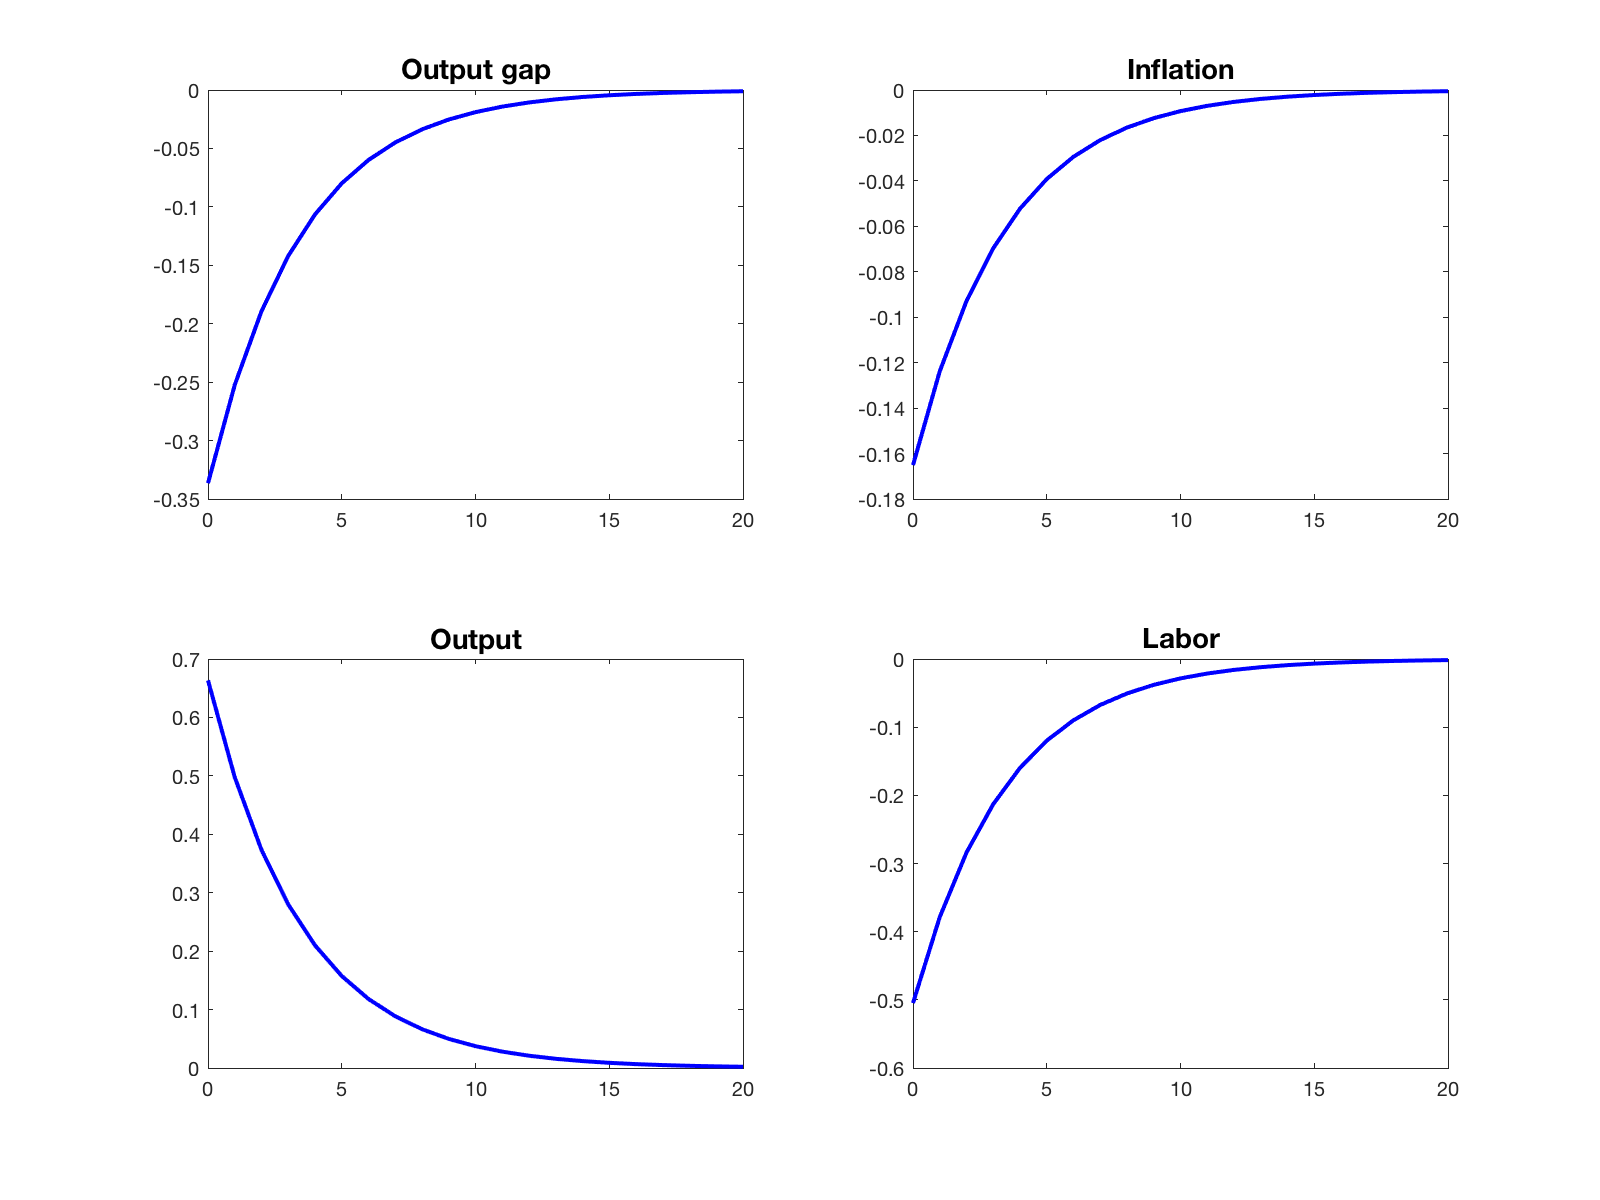
\includegraphics[width=0.75\textwidth]{techshock}
		\caption{Response to 1\% technology shock}
	\end{figure}

    \begin{figure}[H]
    	\centering
    	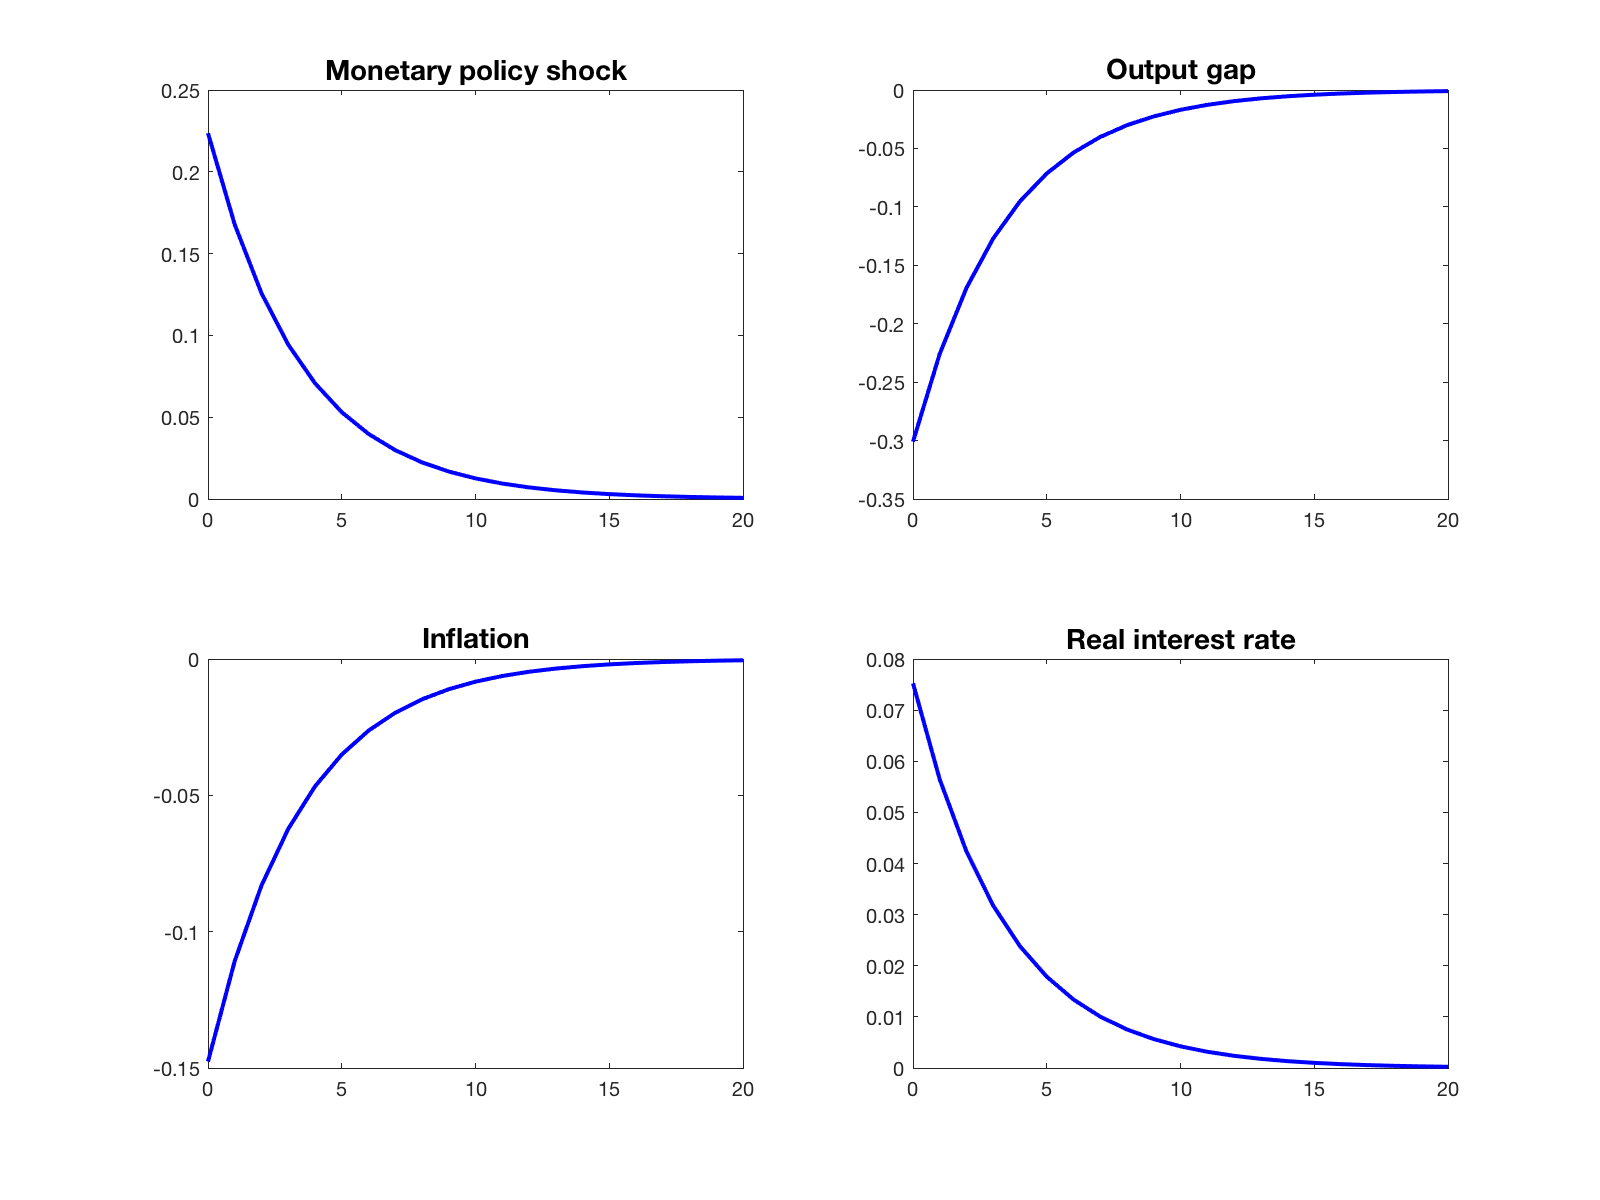
\includegraphics[width=0.75\textwidth]{monetaryshock}
    	\caption{Response to contractionary monetary shock}
    \end{figure}  
\end{enumerate}
\section{Government spending multipliers in the new Keynesian model (Christiano, Eichenbaum and Evans 2012)}
\begin{enumerate}[label = (\alph*)]
	\item The economy is characterized by the following log-linearized equations:
	\begin{align*}
	 \check { C } _ { t } &= E _ { t } \check { C } _ { t + 1} - \frac { 1} { \psi } \left( i _ { t } - E _ { t } \pi _ { t + 1} \right)  \\ 
	 \pi _ { t } &= \beta E _ { t } \pi _ { t + 1} + \kappa \left( \frac { \check {W} } { P } \right)_t ,\quad \kappa = \frac { ( 1- \theta ) ( 1- \beta \theta ) } { \theta }  \\
	\left( \frac { \check{ W } } { P } \right) _ { t } &= \psi \check { C } _ { t } + \frac { 1} { \eta } L _ { t } \\
	\check { Y } _ { t } &= \check { L } _ { t } \\
	\check{ Y }_t &= s_g \check{G}_t + (1-s_g) \check{ C }_t \\
	i_t &= \phi_\pi \pi_t, \quad \phi_\pi > 1
	\end{align*}
	The first equation is a standard Euler equation. The second equation is a recursive formulation of inflation rate, telling us that current inflation is a present value of future marginal costs. The third equation is household's labor supply. The fourth equation denotes aggregate production function. The fifth equation is national account, where $s_g$ is the share the government spending. Finally, the last equtaion implies that the central bank follows the Taylor rule. 
	
	\item The reduced system is characterized as follows: 
	\begin{align*}
	\check{ C }_t &= E_t \check{ C }_{t+1} - \frac{1}{\psi} \left(\phi_\pi \pi_t - E_t\pi_{t+1} \right) \\
	\pi_t &= \beta E_t \pi_{t+1} + \kappa \left( \psi \check{ C }_t + \frac{s_g}{\eta} \check{ G}_t + \frac{(1-s_g)}{\eta} \check{ C }_t \right)
	\end{align*}
	We have two endogenous variables ($\check{ C }_t, \pi_t$) and one exogenous variable ($\check{ G}_t$). 
	
	\item Assume that government spending has the following dynamics: 
	\begin{equation*}
	\check { G } _ { t } = \rho \check { G } _ { t - 1} + \epsilon _ { t } ,\quad \epsilon _ { t } \sim i .i .d .\left( 0,\sigma ^ { 2} \right)
	\end{equation*} 
	Since both $\check{ C }_t$ and $\pi_t$ are jump-variables, the only state variable is $\check{ G}_t$.  $1$ is not a state variable because the model is log-linearized. Since $\check{ C }_{t-1}$ and $\pi_{t-1}$ do not show up in the system, lagged endogenous variables are also not state variables. 
	
	\item Since rational expectation was introduced to the literature, numerous researchers have commented on the multiplicity of solution paths in linear rational expectation models. Since models with inifinite number of solutions which are consistent with rational expectation are evidently unusable, seeking for a solution procedure which can single out a unique, bubble-free solution was a natural flow of the literature. 
	
	McCallum(1983) suggests a solution procedure called the \textit{minimum state variable (MSV) criterion}. Since the multiplicity (or sunspots) arises from redundant state variables which are unnecessary but not formally inconsistent with rational expectations, he suggests to rule out those state variable from the beginning. In our model, the minimum set of state variables is $\{\check{ G }_t\}$. The solution equations for $\check{ C }_t$ and $\pi_t$ are expressed as functions of state variable $\check{ G }_t$:
	\begin{align*}
	\check{ C }_t &= c_g \check{ G}_t \\
	E_t \check{ C }_{t+1} &=c_g \rho \check{ G}_t \\
	\pi_t &= \pi_g \check{ G }_t \\
    E_t \pi_{t+1} & = \pi_g \rho \check{ G }_t	
	\end{align*}
	Plugging in these guessed form of solution equations into the system: 
	\begin{gather*}
	c_g \check{ G}_t = c_g \rho \check{ G}_t - \frac{1}{\psi} \left(\phi_\pi \pi_g \check{ G }_t - \pi_g \rho \check{ G }_t\right) \\
	\pi_g \check{ G }_t = \beta \pi_g \rho \check{ G }_t + \kappa \left( \psi c_g \check{ G}_t + \frac{s_g}{\eta} \check{ G}_t + \frac{(1-s_g)}{\eta} c_g \check{ G}_t \right)
	\end{gather*}
	With some algebraic effort, we get 
	\begin{align*}
	\pi _ { g } &= \frac { \frac { \kappa } { \eta } ( 1- \rho ) s _ { g } } { ( 1- \beta \rho ) ( 1- \rho ) + \frac { \kappa } { \psi } \left[ \psi + \frac { 1} { \eta } \left( 1- s _ { g } \right) \right] \left( \phi _ { \pi } - \rho \right) } \\
	c _ { g } &= \frac { - \frac { \kappa } { \eta \psi } \left( \phi _ { \pi } - \rho \right) s _ { g } } { \left( 1 -  \beta \rho \right) ( 1- \rho ) + \frac { \kappa } { \psi } \left[ \psi + \frac { 1} { \eta } \left( 1- s _ { g } \right) \right] \left( \phi _ { \pi } - \rho \right) }
	\end{align*}
	\item Following the solutioin obtained in (d), 
	\begin{align*}
	\frac{d Y}{d G} =  1 + \frac{d C}{d G} &= 1 + \frac{1-s_g}{s_g} \frac{d \check{ C }}{d \check{ G }} \\
	& = 1 + \frac{c_g (1-s_g)}{s_g} \\
	& = 1 - \frac {  \frac { \kappa } { \eta \psi } \left( \phi _ { \pi } - \rho \right) (1-s _ { g }) } { \left( 1 -  \beta \rho \right) ( 1- \rho ) + \kappa \left[ 1 + \frac { 1} { \eta \psi } \left( 1- s _ { g } \right) \right] \left( \phi _ { \pi } - \rho \right) } \\
	& = 1 - \frac {  \frac { \kappa } { \eta \psi } \left( \phi _ { \pi } - \rho \right) (1-s _ { g }) } { \left( 1 -  \beta \rho \right) ( 1- \rho ) + \kappa(\phi_\pi - \rho) + \frac { \kappa } { \eta \psi } \left( 1- s _ { g } \right)  \left( \phi _ { \pi } - \rho \right) } \\
	& \qquad \text{Let } \frac { \kappa } { \eta \psi } \left( \phi _ { \pi } - \rho \right) (1-s _ { g }) = A \\
	& = 1 - \frac{A}{\left( 1 -  \beta \rho \right) ( 1- \rho ) + \kappa(\phi_\pi - \rho) + A} 
	\end{align*}
	\item Since $\left( 1 -  \beta \rho \right) ( 1- \rho ) + \kappa(\phi_\pi - \rho) >1$, $	dY / dG  < 1$. The government spending multiplier is smaller than one because the Taylor rule effectively stabilizes the inflation, hence cools down the economy.
	\item When $\phi = 0$, the government spending multiplier is:
	\begin{align*}
	\frac{d Y}{d G} &=  1 + \frac{\frac{\kappa}{\eta \phi} \rho(1-s_g)}{(1-\beta \rho)(1-\rho) - \frac{\kappa}{\psi} \left[ \psi + \frac{1}{\eta} (1-s_g) \right] \rho } \\
	& > 1
	\end{align*}
	So the government spending multiplier is larger than 1 even for a very low persistence shock. This is because the monetary policy is not raising nominal interest rate enough to make the real interest rate $r_t = i_t - E_t \pi_{t+1}$ also rise. Since the real interest rate is too low, even a small demand shock can make a ripple effect. 
	
	\item Assuming $\phi_\pi = 0$, or generally any value of $\phi_\pi$ which violates the Taylor principle ($\phi_\pi >1$) is problematic because the model becomes explosive. 
	\item The economy in the ZLB is characterized by the following system of equations: 
	\begin{align*}
	\check { C } _ { t } &= E _ { t } \check { C } _ { t + 1} - \frac { 1} { \psi } \left( i_t - E _ { t } \pi _ { t + 1} \right)  \\ 
	\pi _ { t } &= \beta E _ { t } \pi _ { t + 1} + \kappa \left( \frac { \check {W} } { P } \right)_t ,\quad \kappa = \frac { ( 1- \theta ) ( 1- \beta \theta ) } { \theta }  \\
	\left( \frac { \check{ W } } { P } \right) _ { t } &= \psi \check { C } _ { t } + \frac { 1} { \eta } L _ { t } \\
	\check { Y } _ { t } &= \check { L } _ { t } \\
	\check{ Y }_t &= s_g \tilde{g} + (1-s_g) \check{ C }_t \\
	i_t &= -\bar{i}
	\end{align*}
	The reduced 2-equation system is: 
	\begin{align*}
	\check { C } _ { t } &= E _ { t } \check { C } _ { t + 1} - \frac { 1} { \psi } \left( -\bar{i} - E _ { t } \pi _ { t + 1} \right) \\
	\pi_t &= \beta E_t \pi_{t+1} + \kappa \left( \psi \check{ C }_t + \frac{s_g}{\eta} \tilde{g} + \frac{(1-s_g)}{\eta} \check{ C }_t \right)
	\end{align*}
	Substituting guessed forms of solutions (without constant terms) into the system yields: 
	\begin{align*}
	c_g^{ZLB}\tilde{g} &= p c_g^{ZLB} \tilde{g} - \frac { 1} { \psi } \left( -\bar{i} - p \pi_g^{ZLB} \tilde{g} \right) \\
	\pi_g^{ZLB} \tilde{g} &= \beta p \pi_g^{ZLB} \tilde{g} + \kappa \left( \psi c_g^{ZLB} \tilde{g} + \frac{s_g}{\eta} \tilde{g} + \frac{(1-s_g)}{\eta} c_g^{ZLB}\tilde{g} \right)
	\end{align*}
	Solving the system gives us 
	\begin{align*}
	\pi _ { g } &= \frac { \frac { \kappa } { \eta } ( 1- p ) s _ { g } } { ( 1- \beta p ) ( 1- p ) - \frac { \kappa } { \psi } \left[ \psi + \frac { 1} { \eta } \left( 1- s _ { g } \right) \right] p } \\
	c _ { g } &= \frac { \frac { \kappa } { \eta \psi } p s _ { g } } { ( 1- \beta p ) ( 1- p ) - \frac { \kappa } { \psi } \left[ \psi + \frac { 1} { \eta } \left( 1- s _ { g } \right) \right] p }
	\end{align*}
	\item Following the solutioin obtained in (i), 
	\begin{align*}
	\frac{d Y}{d G} =  1 + \frac{d C}{d G} &= 1 + \frac{1-s_g}{s_g} \frac{d \check{ C }}{d \check{ G }} \\
	& = 1 + \frac{c_g^{ZLB} (1-s_g)}{s_g} \\
	& = 1 + \frac { \frac { \kappa } { \eta \psi } p (1-s_g) } { ( 1- \beta p ) ( 1- p ) - \frac { \kappa } { \psi } \left[ \psi + \frac { 1} { \eta } \left( 1- s _ { g } \right) \right] p }
	\end{align*}
	\item Given $( 1- \beta p ) ( 1- p ) - \frac { \kappa } { \psi } \left[ \psi + \frac { 1} { \eta } \left( 1- s _ { g } \right) \right] p > 0$, the government spending multiplier is always larger than 1. This is because the Taylor rule is not working at the ZLB, so the monetary policy does not stabilize the economy. 
	\item Compare the two government spending multipliers
	\begin{align*}
	\text{in (g): }& \quad 	\frac{d Y}{d G} =  1 + \frac{\frac{\kappa}{\eta \phi} \rho(1-s_g)}{(1-\beta \rho)(1-\rho) - \frac{\kappa}{\psi} \left[ \psi + \frac{1}{\eta} (1-s_g) \right] \rho }\\
	\text{in (k): }& \quad \frac{d Y}{d G} = 1 + \frac { \frac { \kappa } { \eta \psi } p (1-s_g) } { ( 1- \beta p ) ( 1- p ) - \frac { \kappa } { \psi } \left[ \psi + \frac { 1} { \eta } \left( 1- s _ { g } \right) \right] p }
	\end{align*}
	Those two multipliers are the same when $p = \rho$. In (g), monetary policy is ineffective indefinitely. Thus the persistence of the government spending shock determines the size of the multiplier. In (k), on the other hand, the probability of escaping form the ZLB determines the size of the multiplier, since $\rho=1$ as long as the economy is trapped in the ZLB. 
\end{enumerate}

\end{document}
